%========== Document settings ==========
\documentclass[11pt,a4paper,twoside,openany]{report}
\setlength\textwidth{145mm}
\setlength\textheight{247mm}
\setlength\oddsidemargin{14.2mm}
\setlength\evensidemargin{0mm}
\setlength\topmargin{0mm}
\setlength\headsep{0mm}
\setlength\headheight{0mm}
\let\openright=\cleardoublepage

%========== Language settings ==========
\usepackage[main=british,czech]{babel}
\usepackage[utf8]{inputenc}
\usepackage[T1]{fontenc}

%========== Packages =============
\usepackage{stddoc}
\usepackage{circuitikz}

%========== Date format ===============
\newdateformat{monthyeardate}{\monthname[\THEMONTH] \THEYEAR}

%========== Declaration ==========
\newcommand\declarationpage{\clearpage
\vspace*{\fill}
\noindent\textbf{Declaration}\\[0.25cm]
I declare that I completed the presented thesis independently and that all used sources are quoted in accordance with the Methodological instructions that cover the ethical principles for writing an academic thesis.\\
\hrule\vspace*{1cm}

\noindent\textbf{Prohlášení}\\[0.25cm]
\foreignlanguage{czech}{Prohlašuji, že jsem předloženou práci vypracoval samostatně a že jsem uvedl veškeré použité informační zdroje v souladu s Metodickým pokynem o dodržování etických principů při přípravě vysokoškolských závěrečných prací.}\\
\begin{center}
	\begin{minipage}{0.45\textwidth}
		\begin{flushleft}
			V Praze, \hdashrule{3cm}{0.5pt}{2pt}
		\end{flushleft}
	\end{minipage}
	~
	\begin{minipage}{0.45\textwidth}
		\begin{flushright}
			\noindent\begin{tabular}{c}
				\\
				\hdashrule{4cm}{0.5pt}{2pt}\\
				Martin Šimák
			\end{tabular}
		\end{flushright}
	\end{minipage}
\end{center}
\clearpage}

%========== Acknowledgements ==========
\newcommand\acknowledgementspage{\clearpage
\vspace*{\fill}
\noindent\textbf{Acknowledgements}\\[0.25cm]
First and foremost, I would like to thank my supervisor, Jiří Velebil, for his outstanding guidance and his zeal throughout the creation of this thesis. Further, I would like to thank my family and my colleagues, namely Erik Rapp and Karolína Veselá, for their invaluable support.\\
\hrule\vspace*{1cm}

\noindent\textbf{Poděkování}\\[0.25cm]
\foreignlanguage{czech}{Především bych rád poděkoval svému vedoucímu, Jiřímu Velebilovi, za jeho vynikající vedení a za jeho zapálenost a vstřícnost během tvorby této práce. Dále bych rád poděkoval své rodině a svým kolegům, zejména Eriku Rappovi a Karolíně Veselé, za jejich neocenitelnou podporu.}
\clearpage}

%========== Abstract ==========
\newcommand\abstractpage{\clearpage
\noindent\textit{Title:}\\
\textbf{Connections on Differentiable Manifolds}\\[0.25cm]
\textit{Author:} Martin Šimák\\[0.25cm]
\textit{Study programme:} Open Electronic Systems\\[0.25cm]
\textit{Supervisor:} doc. RNDr. Jiří Velebil, Ph.D., Department of Mathematics FEE\\[0.25cm]
\textit{Abstract:}\\
One of the aims of this thesis is to fully introduce a comprehensive differentiable structure on a smooth manifold. To achieve that, we first inspect various aspects of its definition. Further, we introduce a tangent structure on said manifolds, allowing us to locally speak of derivatives and vector fields. This construction naturally results in definitions of a covariant derivative and a connection form, where the former serves as a generalization of a derivative in a direction and the latter as a tool for ``glueing'' tangent spaces together. As a climax of the thesis, we show that the two previously mentioned additional structures on the ambient manifold are equivalent.\\[0.25cm]
\textit{Keywords:} smooth manifolds, tangent structure, covariant derivative, connection\\[0.5cm]
\noindent\textit{Název práce:}\\
\textbf{Konexe na diferencovatelných varietách}\\[0.25cm]
\textit{Autor:} Martin Šimák\\[0.25cm]
\textit{Studijní program:} Otevřené elektronické systémy\\[0.25cm]
\textit{Vedoucí:} doc. RNDr. Jiří Velebil, Ph.D., katedra matematiky FEL\\[0.25cm]
\textit{Abstrakt:}\\
\foreignlanguage{czech}{Jedním z cílů této práce je v plném měřítku uvést rozsáhlou diferenciální strukturu na hladké varietě. Abychom toho dosáhli, prozkoumáme nejprve jednotlivé aspekty její definice. Dále na varietách uvedeme tečnou strukturu, jenž nám umožňuje lokálně hovořit o derivacích a vektorových polích. Tato konstrukce přirozeně vyúsťuje v definice kovariantní derivace a konexe, přičemž první z pojmů slouží jakožto zobecnění derivace ve směru a druhý jakožto nástroj pro \uv{slepování} tečných prostorů. Jako vyvrcholení práce ukážeme, že tyto dvě dodatečné struktury na varietě jsou ekvivalentní.}\\[0.25cm]
\textit{Klíčová slova:} hladké variety, tečná struktura, kovariantní derivace, konexe\\[0.5cm]
\clearpage}

%========== Bibliography ==========
\bibliographystyle{abbrvnat}

%========== Custom commands ==========
\newcommand{\Tx}{\mathrm{Tx}}
\newcommand{\Rx}{\mathrm{Rx}}

%========== Draft settings ==========
\usepackage{lipsum}


\makeindex
\begin{document}

    \pagenumbering{gobble}
    
    %========== Title page ==========
    % Suppress displaying the page number on the title page + count the following page as page 1 (not used)
    \begin{titlepage}
        % Define a new command for horizontal lines, change thickness here
\newcommand{\HRule}{\rule{\linewidth}{0.5mm}}
\center

%========== Header ==========
\textsc{\LARGE Czech Technical University in Prague,\\Faculty of Electrical Engineering}\\[1.5cm]
\textsc{\Large Master's thesis}\\[0.5cm]

%========== Title ==========
\HRule\\[0.6cm]
{\huge\bfseries Dual Circularly Polarized Waveguide Antenna}\\[0.3cm] % Title of your document
\HRule\\[1.5cm]

%========== Authors ==========
\begin{minipage}{0.45\textwidth}
    \begin{flushleft}
        \large
        \textit{Author}\\
        M. \textsc{Šimák}\\
        \textsc{Department of Electromagnetic Field}
    \end{flushleft}
\end{minipage}
~
\begin{minipage}{0.45\textwidth}
    \begin{flushright}
        \large
        \textit{Supervisor}\\
        doc. Ing. P. \textsc{Hazdra}, Ph.D.\\
        \textsc{Department of Electromagnetic Field}
    \end{flushright}
\end{minipage}

%========== Logo ==========
% Position at 3/4 of the screen
\vfill\vfill\vfill

\includegraphics[width=0.3\textwidth]{src/ctu_logo_black.jpg}

%========== Date ==========
\vfill\vfill
{\large\monthyeardate\today}
% Push the date up 1/4 of the remaining page
\vfill
    \end{titlepage}

    %========== Blank page ==========
    \newpage\blankpage

    % %========== Assignment ==========
    % 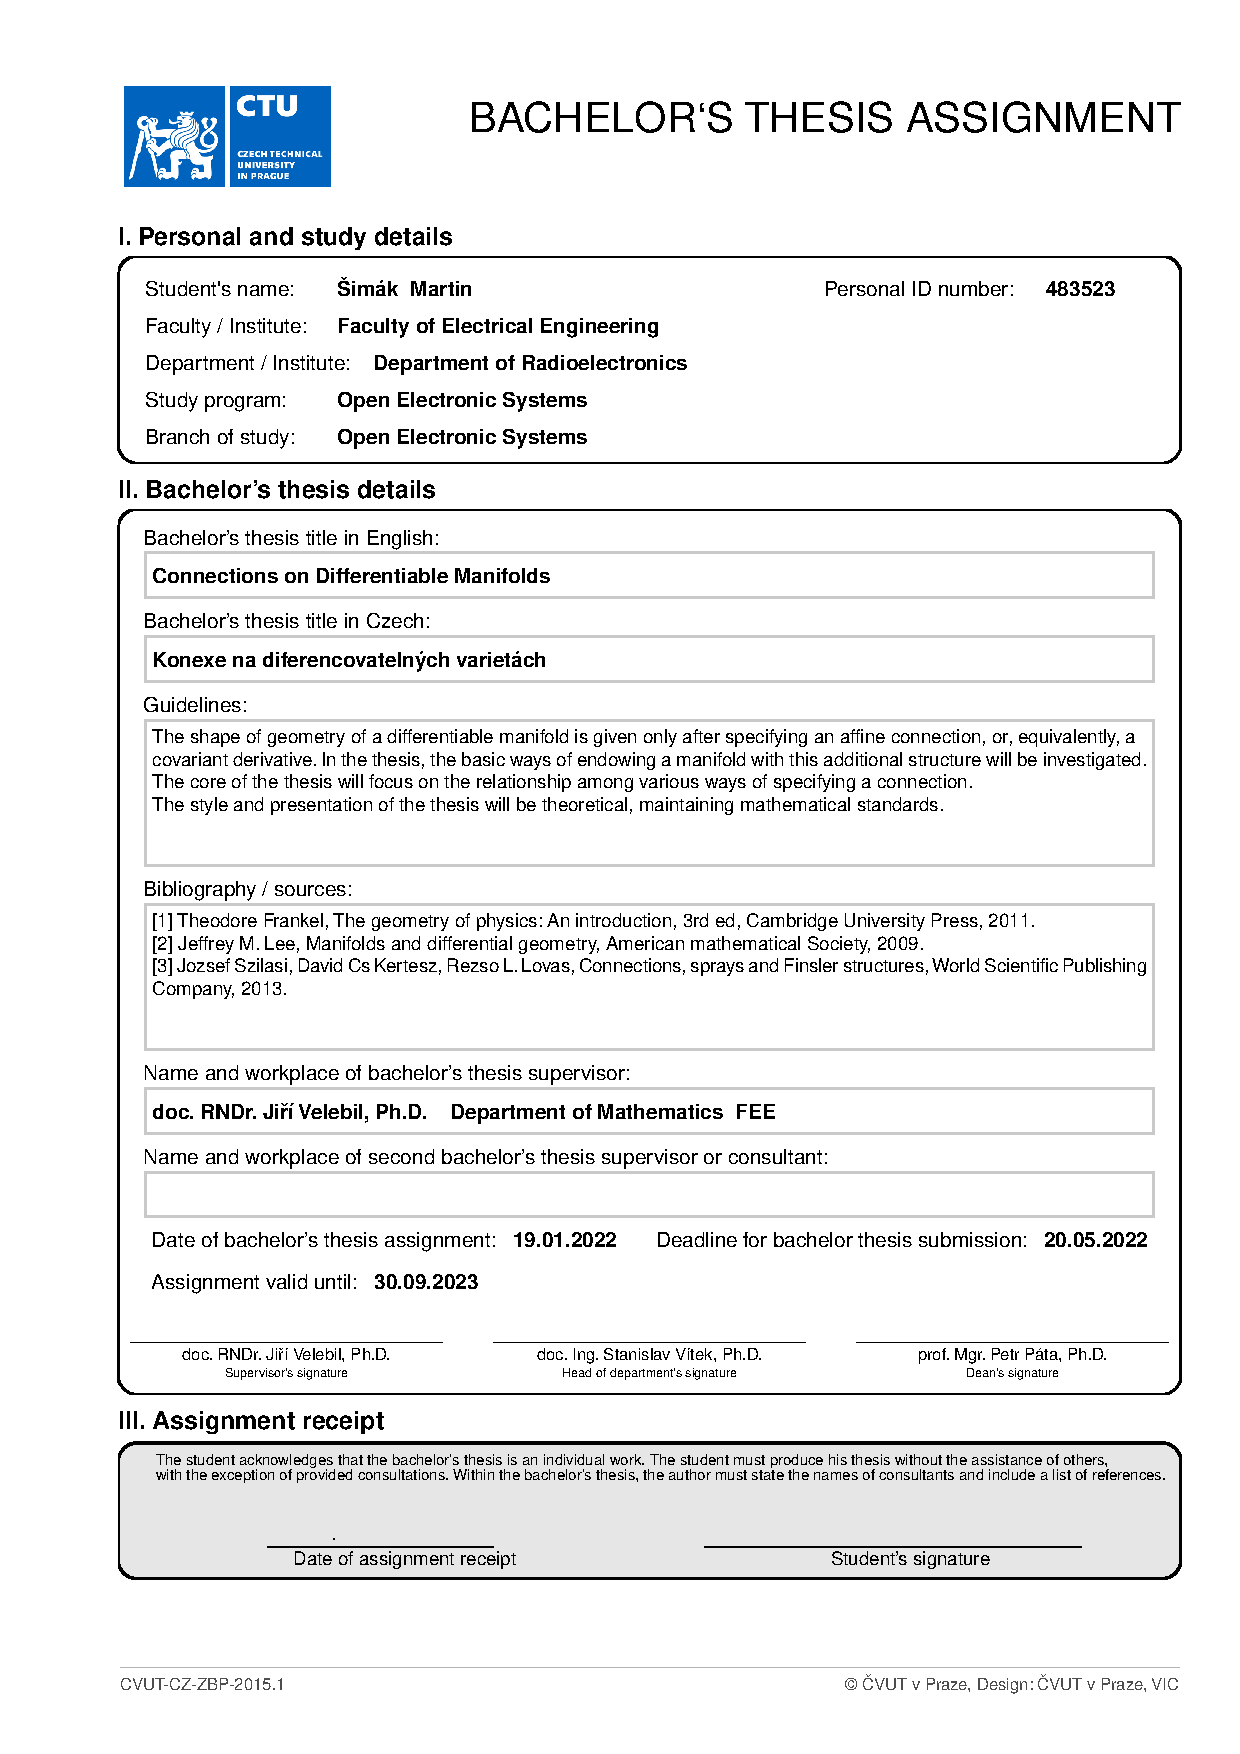
\includepdf[pages=-]{src/assignment.pdf}

    % %========== Blank page ==========
    % \newpage\blankpage

    % Start counting pages in roman numerals
    \pagenumbering{roman}

    % %========== Declaration ==========
    % \declarationpage

    % %========== Acknowledgements ==========
    % \acknowledgementspage

    % %========== Abstract ==========
    % \abstractpage

    % Start counting pages in arabic numerals
    \pagenumbering{arabic}

    %========== Table of contents ==========
    \tableofcontents

    %========== Introduction ==========
    % This is just a very vague introduction for the thesis project which is to be rewritten later on.
    \chapter*{Introduction}
    \label{chap:introduction}
    \addcontentsline{toc}{chapter}{\nameref{chap:introduction}}
    
    \lipsum[1-2]

    \paragraph*{Synopsis.} In \textbf{Chapter~\ref{chap:first-chapter}}, \lipsum[3]

    \paragraph*{Methodology.} \lipsum[4]


    %========== Chapter 1: First chapter ==========
    \chapter{Chapter}
    \label{chap:first-chapter}

    \lipsum[5-6] Random citation~\cite{kracek-mazanek:power-balance-of-inductive-wireless-power-transfer}.

    \section{Section}
    \label{sec:first-section}

        \lipsum[7-9]

    
    %========== Conclusion ==========
    \chapter*{Conclusion}
    \label{chap:conclusion}
    \addcontentsline{toc}{chapter}{\nameref{chap:conclusion}}
    
    \lipsum[10-13]

    %========== Bibliography ==========
    \bibliography{bibliography}
	
    % %========== Index ==========
	% \printindex

\end{document}
